\chapter{Betriebsschwingungsanalyse - HKA}
\label{sec: Hauptkapitel 3}

\section{Aufgabenstellung}
    % Grundziel
    %----------
    Auch bei dieser Laboraufgabe soll eine Betriebsschwingungsanalyse
    durchgeführt werden. Diesmal ist das Zeitsignal jedoch an mehreren, vorher
    definierten, Punkten an der Tragfläche aufzunehmen. Für das Schleppen des
    Motors kann der Versuchsaufbau der vorhergehenden Laborübung verwendet
    werden.
    \\
    %----------------------------------------------------------------------------

    % Ausdetaillierung
    %-----------------
    \noindent
    Nach Aufnahme der Zeitsignale soll eine Hauptkomponentenanalyse (HKA)
    durchgeführt werden. Dies soll einmal für das gesamte Signal gemacht werden.
    In einem 2. Schritt soll die Rampe in 10 gleich große Intervalle unterteilt
    werden. Zu jedem dieser Zeitintervalle gilt es, anschließend eine HKA
    durchzuführen.
%================================================================================

\section{Versuchsaufbau}
    % Versuchsaufbau genauer beschrieben
    Der Versuchsaufbau entspricht dem in Kapitel 3 beschriebenen Aufbau. Der einzige 
    Utnerschied besteht darin, dass für die Hauptkomponentenanalyse die Daten aller 
    vier Sensoren verwendet werden. 
    \\

    \noindent
    Der für die HKA verwendete Code ist im Anhang zu finden.
%================================================================================

\section{Ergebnisse}
    \subsection{HKA für den gesamten Datensatz}
        Die Hauptkomponentenanalyse wurde zunächst für den gesamten aufgezeichneten
        Datensatz durchgeführt. Die Ergebnisse sind in Abbildung \ref{fig: HKA gesmat} dargestellt.
        Da sich die Sensoren ausschließlich auf dem Tragflügel befinden, wurde 
        eine 2D-Darstellung gewählt, um die Eigenvektoren übersichtlicher und besser 
        interpretierbar darzustellen.

        % Bild - HKA Gesamt
        %--------------------------------------
        \begin{figure}[H]
            \centering
            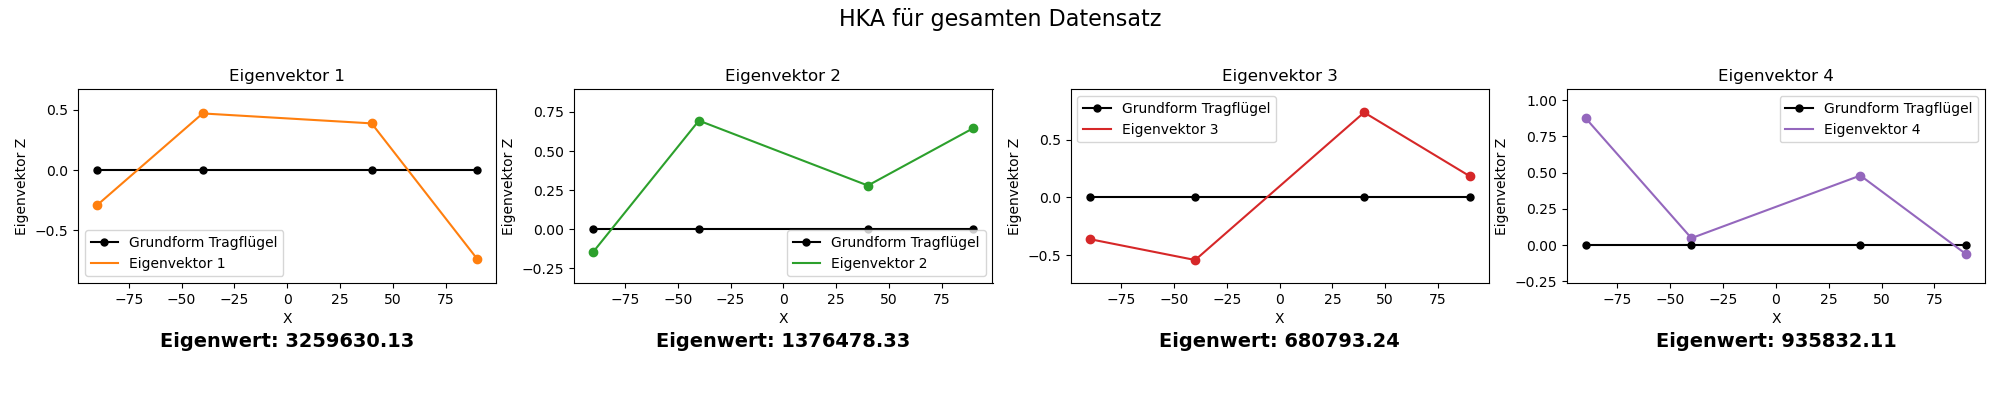
\includegraphics[width=0.95\textwidth]{HKA_Gesamt.png}
            \caption{HKA kompletter Datensatz}
            \label{fig: HKA gesmat}
        \end{figure}

        \noindent
        Die HKA für den gesamten Datensatz zeigt die vier berechneten Eigenvektoren sowie deren 
        zugehörige Eigenwerte. Da nur vier Sensoren auf dem Tragflügel platziert sind, können 
        auch nur vier Eigenvektoren dargestellt werden. Die schwarze Linie stellt die Grundform 
        des Tragflügels dar, während die farbigen Linien die jeweiligen Eigenmoden repräsentieren.
        \\

        \noindent
        Aus den Eigenwerten wird ersichtlich, dass der zweite Mode mit dem größten Eigenwert 
        die dominante Schwingungsform des Tragflügels ist und den größten Anteil an der 
        Gesamtbewegung trägt. Die anderen höher frequenten Moden sind weniger stark ausgeprägt.
    \subsection{HKA für den unterteilten Datensatz}
        Um zeitliche Veränderungen der Schwingungscharakteristik zu untersuchen, wurde die Rampe 
        in zehn gleich große Zeitintervalle unterteilt. Für jedes dieser Intervalle wurde eine 
        separate HKA durchgeführt. 

        \noindent
        Die Ergebnisse dieser schrittweisen Analyse sind in den nachfolgenden Abbildungen dargestellt. 
        Durch den Vergleich der Eigenvektoren in den einzelnen Zeitabschnitten lassen sich mögliche 
        Änderungen in der Schwingungscharakteristik während der Versuchsdurchführung erkennen.

        % Bilder - HKA für einzelne Zeitintervalle
        %--------------------------------------% Bilder - HKA für einzelne Zeitintervalle
        % Bild - HKA Intervall 1
        %--------------------------------------
        \begin{figure}[H]
            \centering
            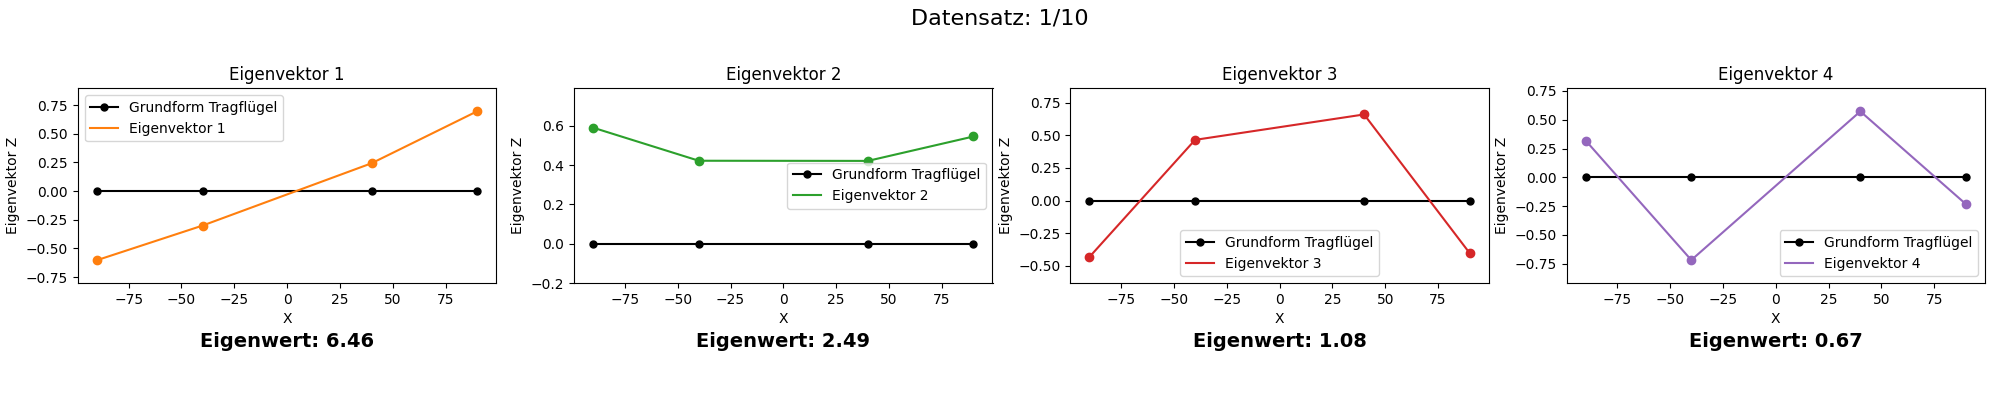
\includegraphics[width=0.95\textwidth]{Datensatz_1.png}
            \caption{HKA - Intervall 1}
            \label{fig: HKA_intervall_1}
        \end{figure}

        % Bild - HKA Intervall 2
        %--------------------------------------
        \begin{figure}[H]
            \centering
            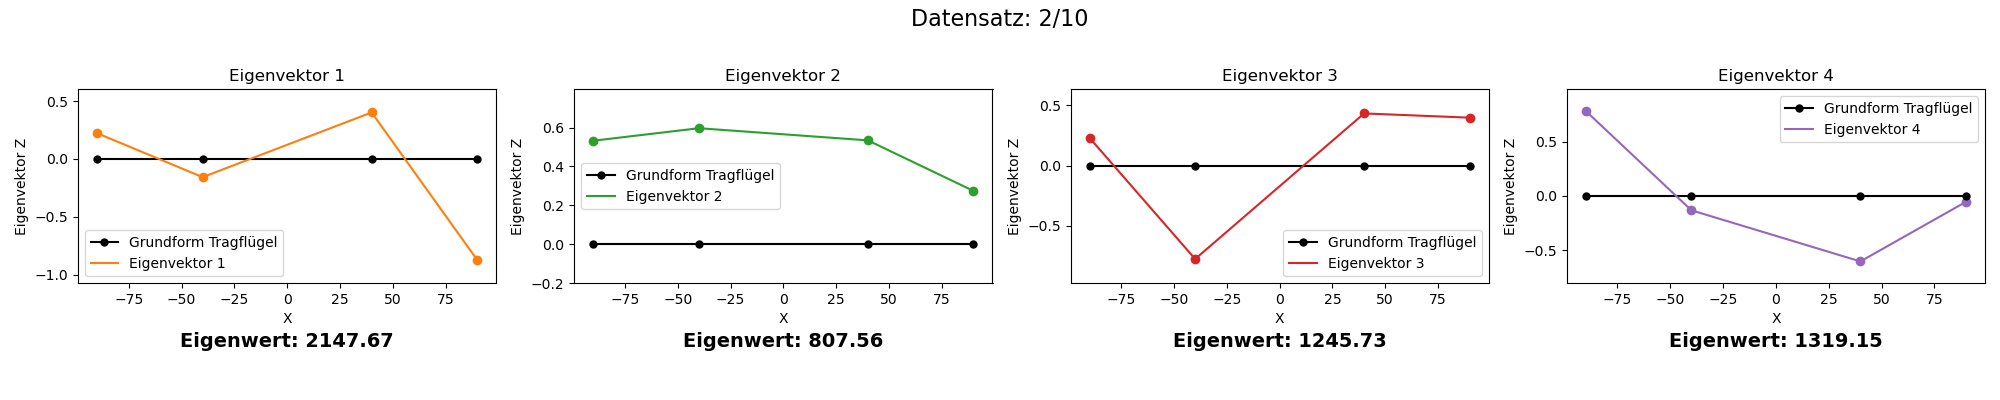
\includegraphics[width=0.95\textwidth]{Datensatz_2.png}
            \caption{HKA - Intervall 2}
            \label{fig: HKA_intervall_2}
        \end{figure}

        % Bild - HKA Intervall 3
        %--------------------------------------
        \begin{figure}[H]
            \centering
            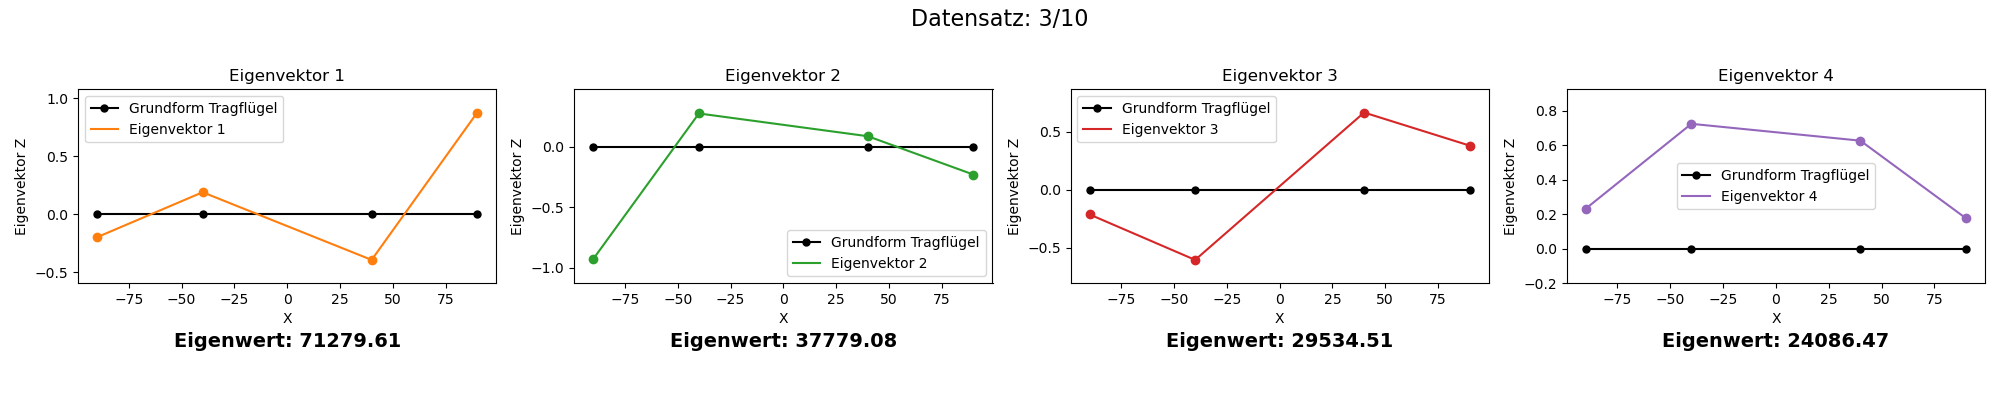
\includegraphics[width=0.95\textwidth]{Datensatz_3.png}
            \caption{HKA - Intervall 3}
            \label{fig: HKA_intervall_3}
        \end{figure}

        % Bild - HKA Intervall 4
        %--------------------------------------
        \begin{figure}[H]
            \centering
            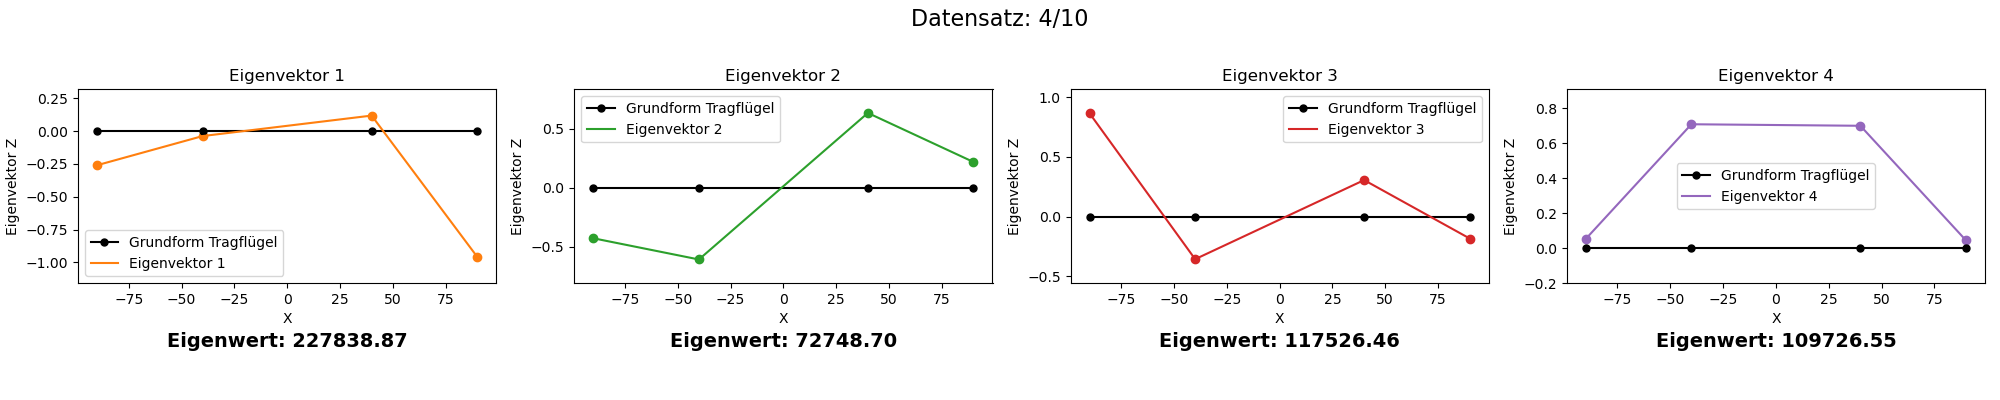
\includegraphics[width=0.95\textwidth]{Datensatz_4.png}
            \caption{HKA - Intervall 4}
            \label{fig: HKA_intervall_4}
        \end{figure}

        % Bild - HKA Intervall 5
        %--------------------------------------
        \begin{figure}[H]
            \centering
            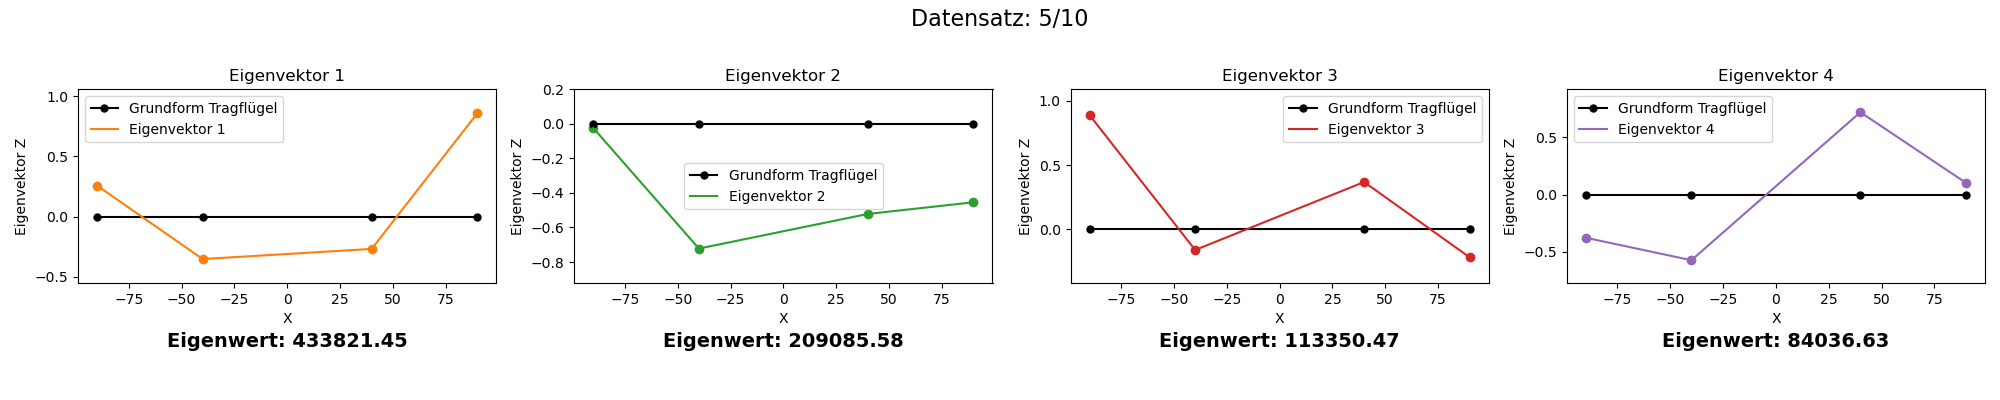
\includegraphics[width=0.95\textwidth]{Datensatz_5.png}
            \caption{HKA - Intervall 5}
            \label{fig: HKA_intervall_5}
        \end{figure}

        % Bild - HKA Intervall 6
        %--------------------------------------
        \begin{figure}[H]
            \centering
            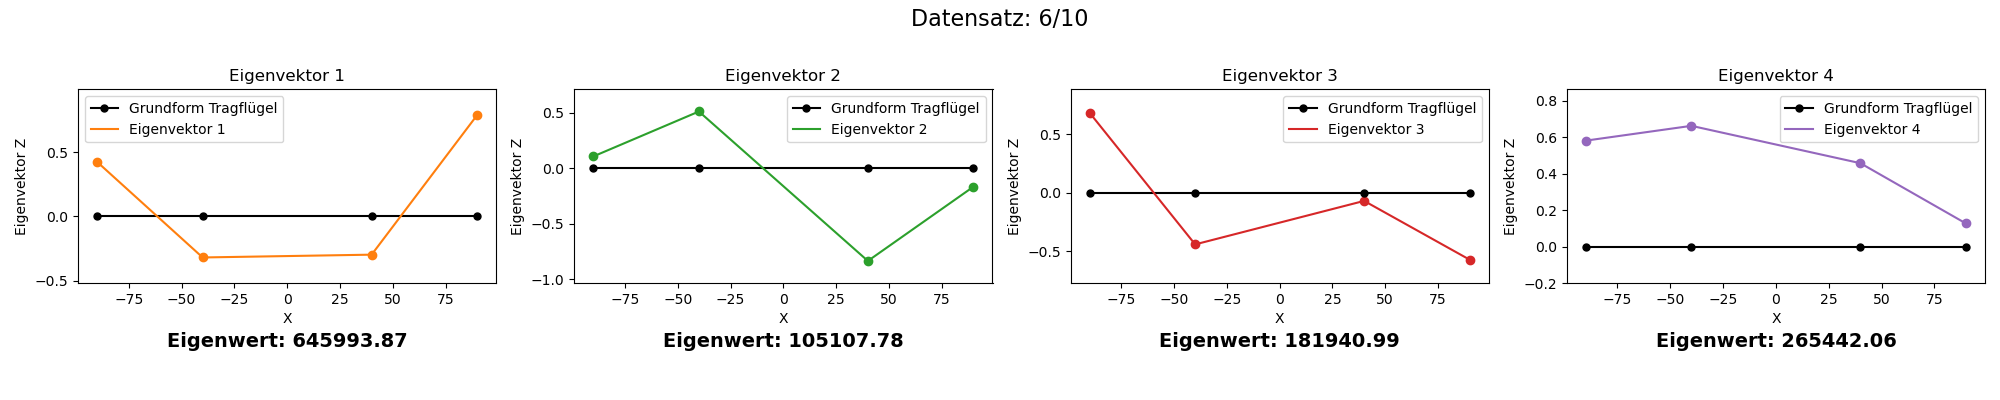
\includegraphics[width=0.95\textwidth]{Datensatz_6.png}
            \caption{HKA - Intervall 6}
            \label{fig: HKA_intervall_6}
        \end{figure}

        % Bild - HKA Intervall 7
        %--------------------------------------
        \begin{figure}[H]
            \centering
            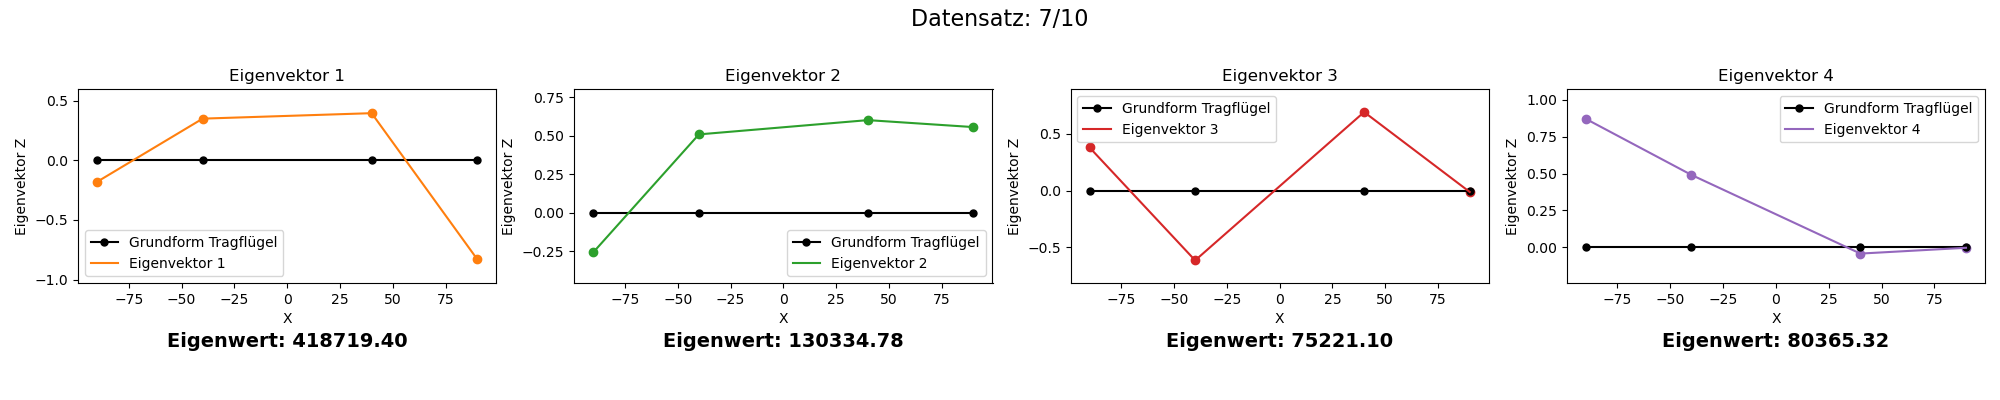
\includegraphics[width=0.95\textwidth]{Datensatz_7.png}
            \caption{HKA - Intervall 7}
            \label{fig: HKA_intervall_7}
        \end{figure}

        % Bild - HKA Intervall 8
        %--------------------------------------
        \begin{figure}[H]
            \centering
            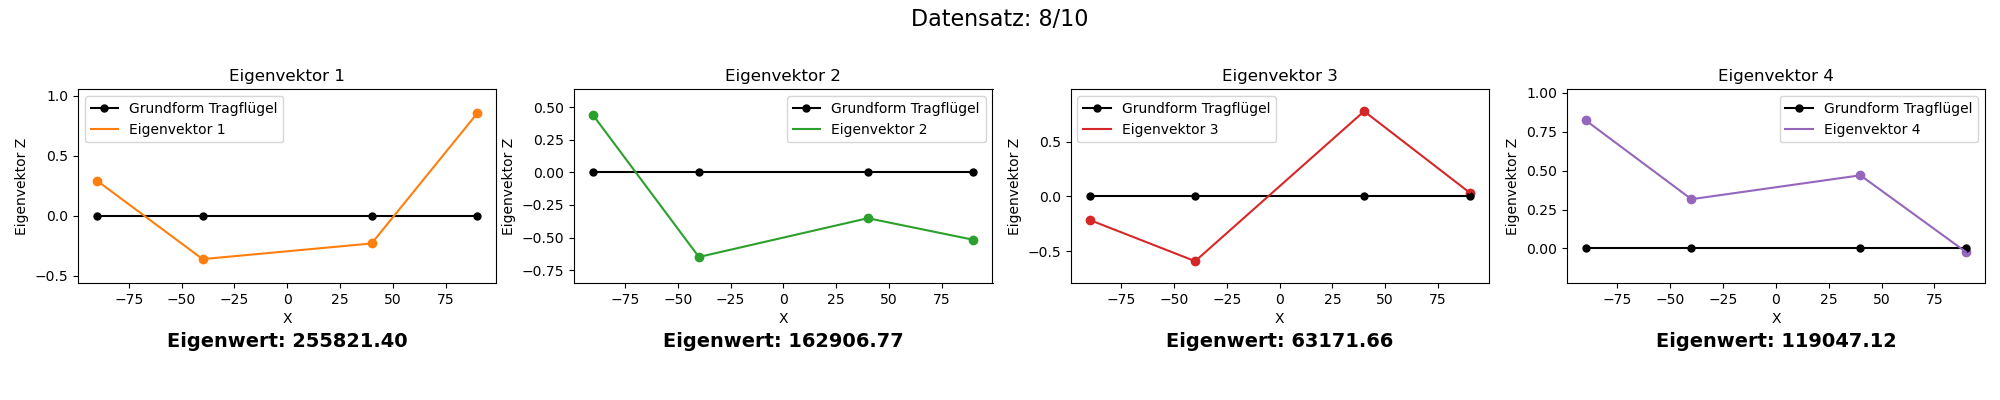
\includegraphics[width=0.95\textwidth]{Datensatz_8.png}
            \caption{HKA - Intervall 8}
            \label{fig: HKA_intervall_8}
        \end{figure}

        % Bild - HKA Intervall 9
        %--------------------------------------
        \begin{figure}[H]
            \centering
            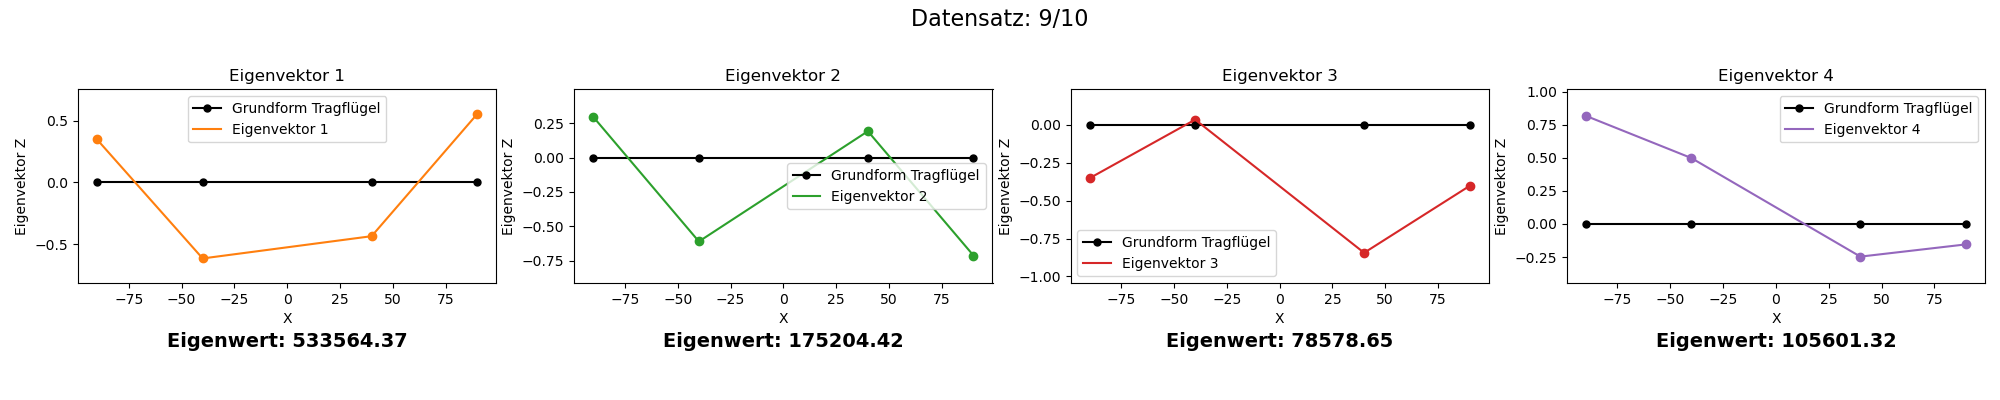
\includegraphics[width=0.95\textwidth]{Datensatz_9.png}
            \caption{HKA - Intervall 9}
            \label{fig: HKA_intervall_9}
        \end{figure}

        % Bild - HKA Intervall 10
        %--------------------------------------
        \begin{figure}[H]
            \centering
            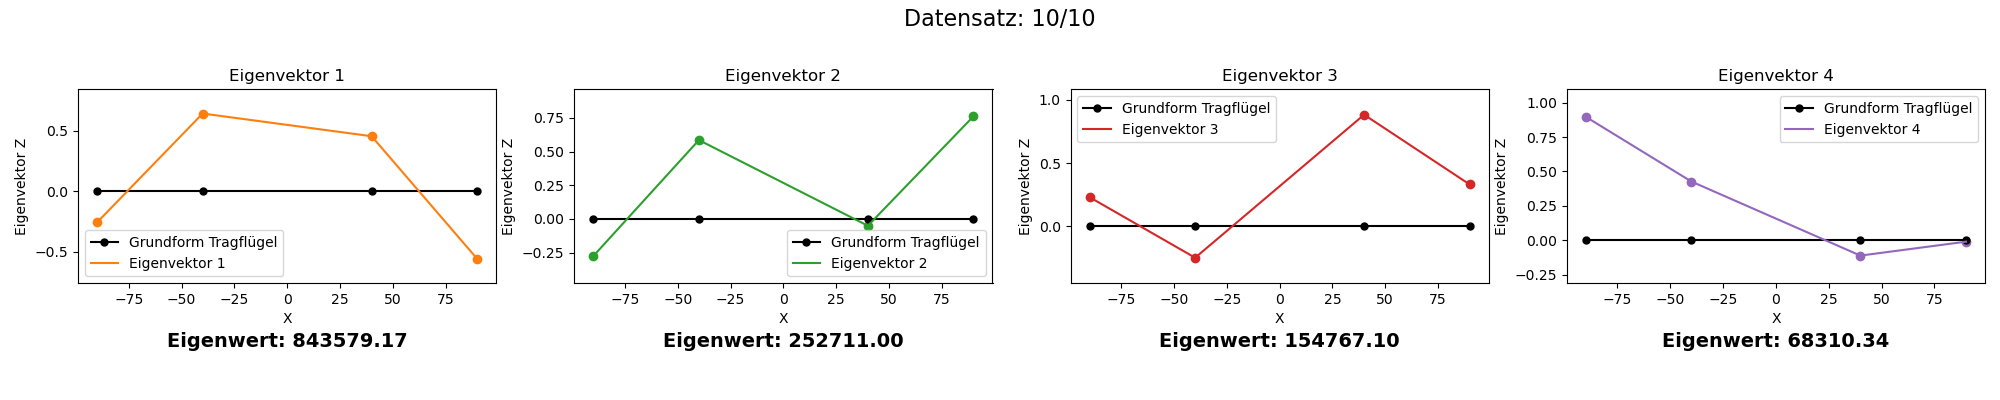
\includegraphics[width=0.95\textwidth]{Datensatz_10.png}
            \caption{HKA - Intervall 10}
            \label{fig: HKA_intervall_10}
        \end{figure}

        \noindent
        Die Ergebnisse der HKA für die zehn Zeitintervalle zeigen, wie sich die dominanten 
        Schwingungsmoden über die Zeit verändern. Im ersten Intervall \ref{fig: HKA_intervall_1} 
        ist der dominante Eigenvektor der Mode 1, welche einer Starrkörperbewegung entspricht. 
        Dies ist zu erwarten, da in diesem frühen Zeitabschnitt vorwiegend niederfrequente 
        Schwingungen auftreten. Mit zunehmender Zeit verändern sich die dominanten Moden. 
        In späteren Intervallen nehmen die Eigenwerte der höheren Moden zu, was darauf 
        hinweist, dass höherfrequente Schwingungen stärker ausgeprägt sind. 